In this section the results will be presented, explained and discussed.
Starting with physical measurements and material properties.
Followed by the presentation of the results obtained by optimization and exploration with the \gls{emma} method. 
Finally, alternative regression methods were applied to the data and the results are compared with the results of the \gls{emma} method. 

%%%%%%%%%%%%%%%%%%%%%%%%%%%%%%%%%%%%%%%%%%%%%%%%%%%%%%%%%%%
%%%%%%%%%%%%%%%%%%%%%%%%%%%%%%%%%%%%%%%%%%%%%%%%%%%%%%%%%%%
\section{Material Properties of the Produced Layers}
\label{sec:res-mat}
%\todo{of what?}
%\subsection{Solution}
%%%%%%%% AQUATIC AQUEOUS
As already indicated in the experimental section the aqueous recipe adopted from Anwar et al.~\cite{Anwar2017} failed to produce a homogeneous layer of \gls{zro}.
The aqueous solution started out as opaque slurry in contrast to the buthanolic recipe which became opaque only after degrading. 
%\td{Die wässrige Lösung hatte direkt nach erzeugung viskose und undurchsichtige Eigenschaften - im Gegensatz zu der anderen Lösung, welche erst nach Stunden von klar auf undurchsichtig umschwenkte.}
%The solution was opaque from the beginning and 
Furthermore, the resulting layers were patchy and laced with cracks (see figure~\ref{fig:sem-old}). 
Altering the ratio of ingredients, adjusting pH (by adding \gls{naoh}, \gls{h2so4} or \gls{hcl}) or adding \gls{sds} as surfactant did not increase the measured resistance through the resulting \gls{zro} layers. 
% ../../Data/SEM/SEM_2020_11_10_Old_Recipes/10_2L_19.tif
% ../../Data/SEM/SEM_2020_11_19_Old_Recipes/71_SL_NT4_11.tif
Even after the consecutive application of two layers, 
there was no significant improvement and the \gls{sem} images (see figure~\ref{fig:sem-old}) 
showed highly inhomogeneous deposition, with deposited  areas next to other areas where the conductive substrate (ITO or FTO) can be clearly seen  uncoated.
%reminded rather of a sparse crust than of a film. 
%It is assumed that the solution was far from the optimum for a sol-gel process. 
%
Figure~\ref{fig:sem-old} shows a typical detail view of \gls{zro} (dark) on top of \gls{fto} (finely polycrystalline). 
%These were the results of a single (figure~\ref{fig:sem-old1}) and double (figure~\ref{fig:sem-old2}) "layer" of the aqueous recipe. 
Large cracks, non-coated areas and inhomogeneity were 
%part of (ausmachen) 
shared characteristics among 
all samples created with the aqueous recipe. 
%even after several/multiple/various alteration to the recipe. 

\begin{figure}[bht]
    \centering
    \begin{subfigure}{.45\textwidth}
        \centering
        %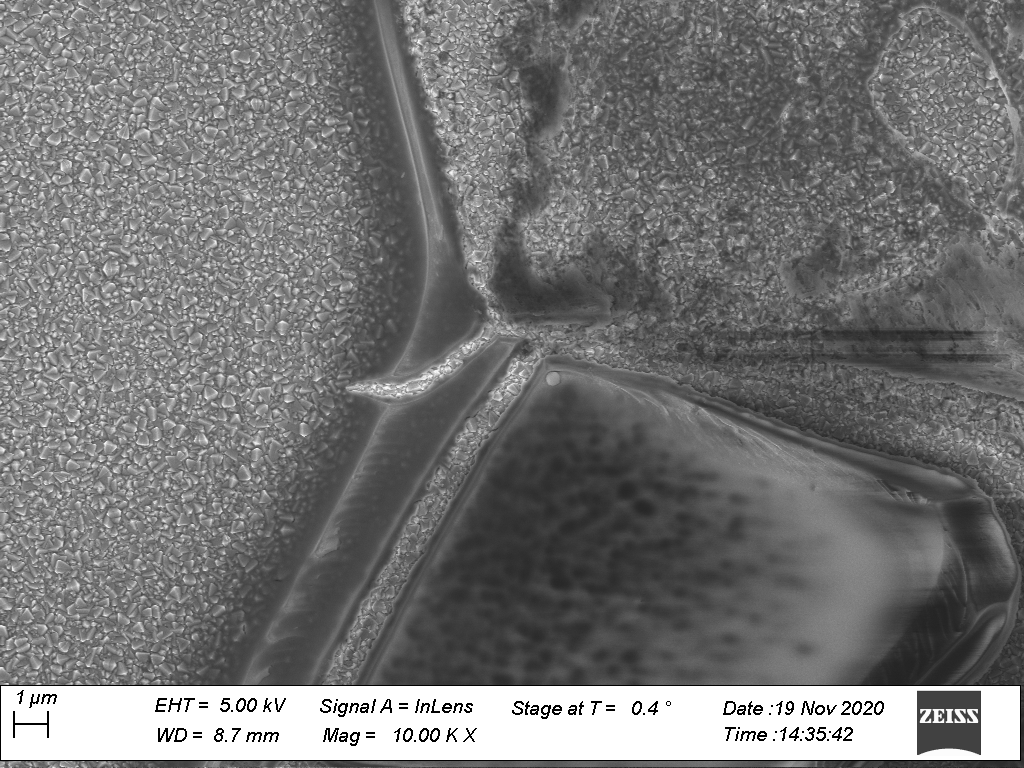
\includegraphics[width=.79\textwidth]{Pics/sem/071_fto_old_1x1F.png}
        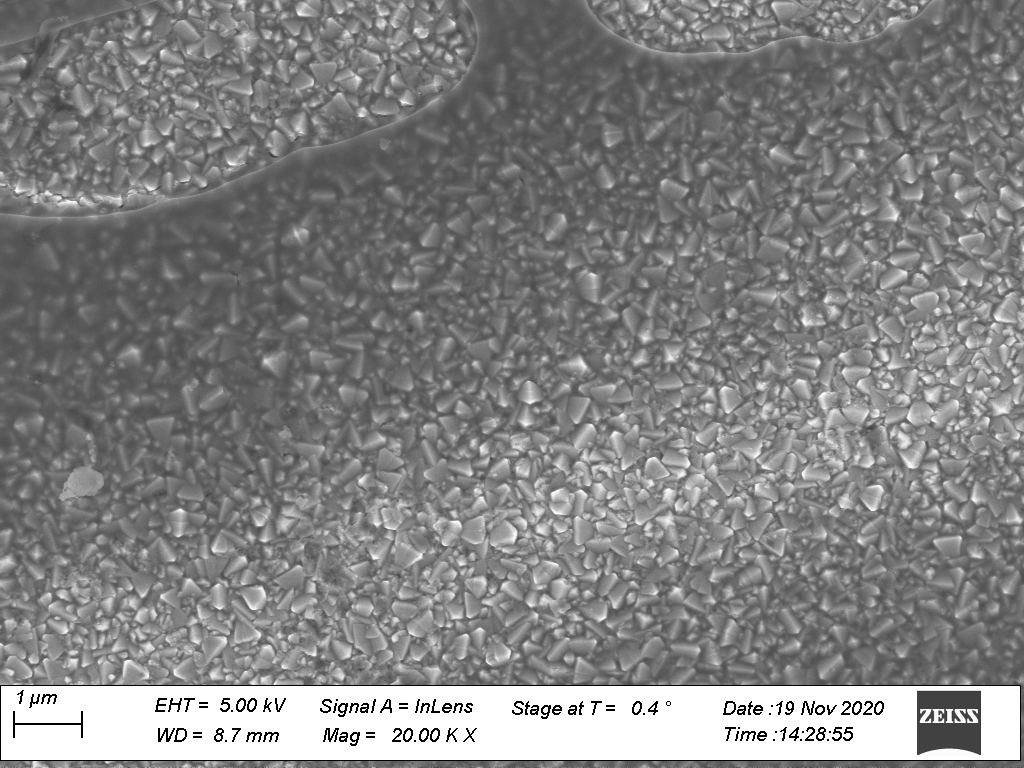
\includegraphics[width=.99\textwidth]{Pics/sem/071_fto_old_2x.png}
		\caption{}%SEM picture of \gls{zro} produces by H2O solution} 
		\label{fig:sem-old}
    \end{subfigure}
    \begin{subfigure}{.45\textwidth}
        \centering
        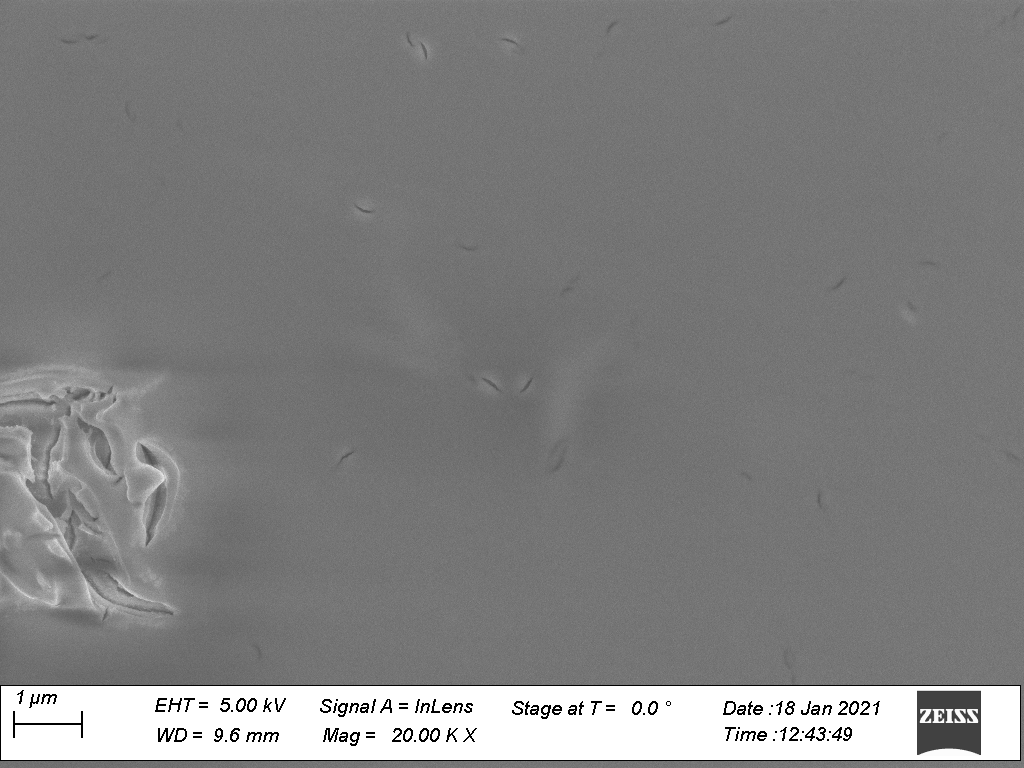
\includegraphics[width=.99\textwidth]{Pics/sem/147_steel_ph_10x.png}
		\caption{}%SEM picture of \gls{zro} produced by buoh solution} 
		\label{fig:sem-ph}
    \end{subfigure}
    \begin{subfigure}{.45\textwidth}
        \centering
        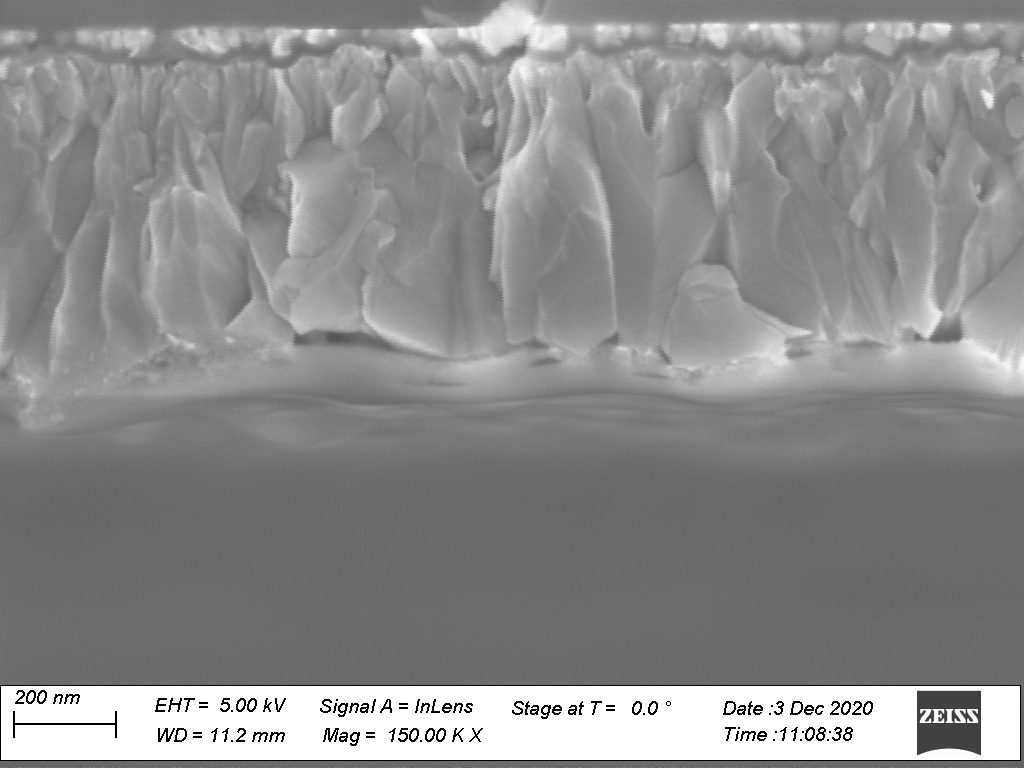
\includegraphics[width=.99\textwidth]{Pics/sem/115_fto_cs_1x.png}
		\caption{}%115 fto cs 5x} 
		\label{fig:sem-cs1}
    \end{subfigure}
    \begin{subfigure}{.45\textwidth}
        \centering
        %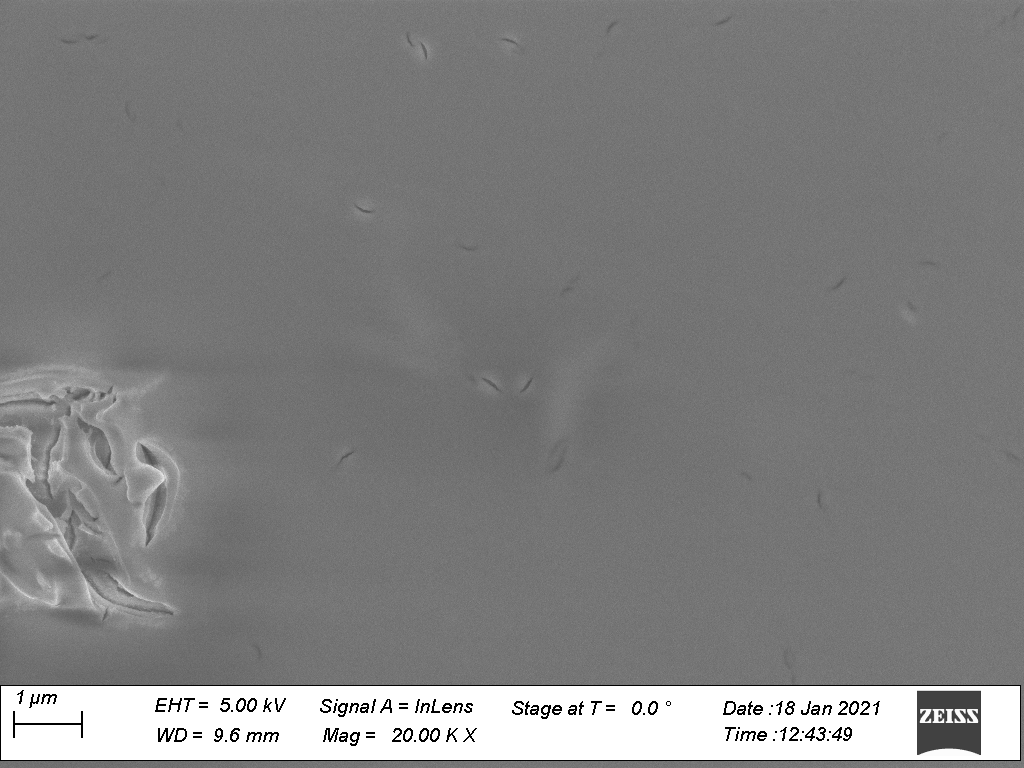
\includegraphics[width=.8\textwidth]{Pics/sem/147_steel_ph_10x.png}
        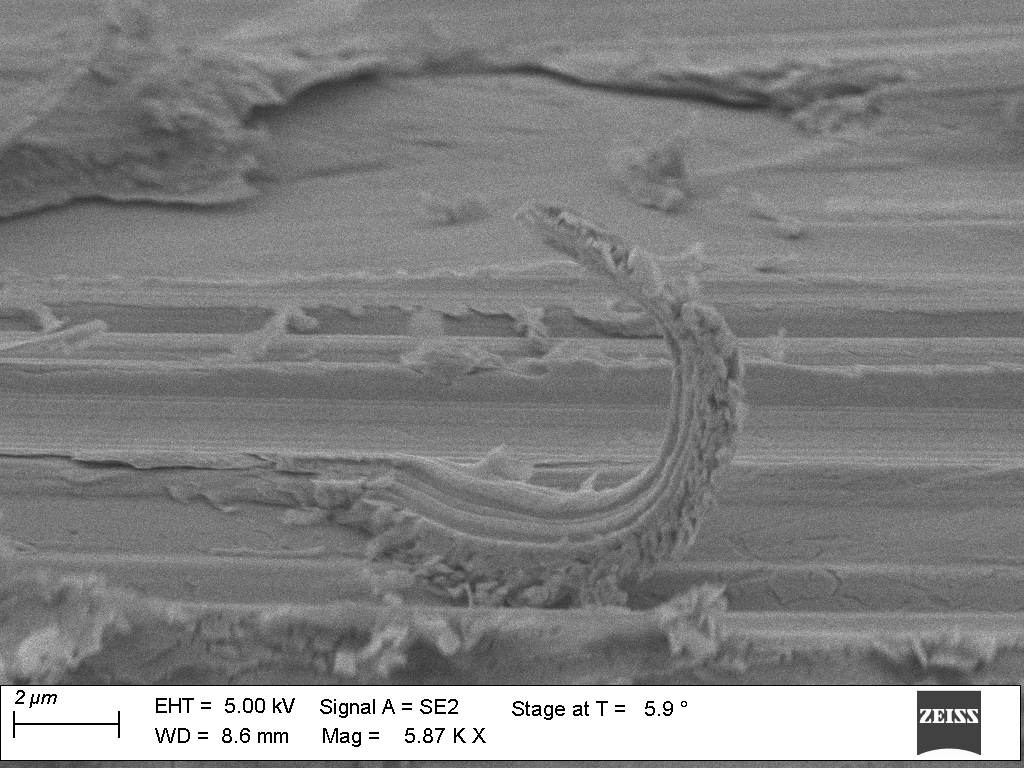
\includegraphics[width=.99\textwidth]{Pics/sem/150_steel_cs_2Fx5.png}
		\caption{}%150 steel 2Fx5} 
		\label{fig:sem-cs2}
    \end{subfigure}
	\caption{
		SEM images of \gls{zro}:
		(a) \gls{zro} produces by 2 layers aqueous solution on \gls{fto}
		(b) 10 layers of \gls{zro} on steel substrate
		(c) cross section of crack of 5 layers of \gls{zro} on \gls{fto}
		(d) side view of scratched \gls{zro} on steel substrate
		%SEM images of \gls{zro} on top of \gls{fto} (a,c) and \gls{zro} on steel (b,d) \td{find bu sol on fto and show only steel}} 
		\label{fig:sem}
	}
\end{figure}
\enlargethispage{-\baselineskip}

The sol-gel recipe reported by Hu et al.\cite{Hu2016} and further optimzed, led to improved results (see section~\ref{sec:exp-sol-bu}). 
%
Figure~\ref{fig:sem-ph} shows a top view of 10 layers of the buthanolic solution on top of a steel substrate. 
%%%% PIN HOLES
The large irregularity on the bottom left could depict a pin hole, a hole in the layer that reaches to the substrate. 
These irregularities are rather the exception. 
Alternatively, the small, hardly visible cracks spread across the surface could depict such pin holes. 
% These - I think - are rather only one layer deep irregularities since they are so prevalent and hardly any pin holes were electrically observed on similar samples. \todo{where is the evidence?}

%%%%%% STABILITY
As soon as the solution showed initial cloudiness, it was declared as unstable and used no more for \gls{db}. %\td{(coating! DB = deutsche Bahn ... ist mir schon vorher aufgefallen)}
The solution becoming opaque indicated build-up of precipitation and was not further used.
The visually asserted stability of the solution could be increased a lot by replacing the stabilizing agent \gls{acoh} with \gls{ipo}.
A \gls{1f} and a \gls{4f} solution with \gls{acoh} - sealed with Parafilm - was stable for approximately \h{24} and \h{2}, respectively.
%192 was first with IPOH
Whereas a \gls{4f} solution with \gls{ipo} as stabilizing agent stayed stable for circa \h{96}. 
An increase of the \gls{zrpro} concentration accelerates the aging process of the solution.
%\td{what is this aging process chemically? oxidation, hydrolization?}.
The aging process was accelerated by absence of proper sealing.
\td{The aging process dependends on the water in the air corresponding to an hyrolization process\cite{Hu2016}.}
%
The introduction of \gls{ipo} into the recipe allowed higher concentrated solutions to be practicable 
as they could be stored until the next day, instead of producing a new, separate solution for each day.
%
It was found that after a \gls{4f} \gls{acoh} solution has 
%aged beyond cloudiness 
shown precipitation (became opaque)
the addition 50\% of the volume in \gls{ipo} can even reverse the aging effect for a respectable amount of time. 
This effect is not only due to dilution as additional solvent (\gls{buoh}) did not re-stabilize the solution, 
even after 5 fold dilution. 
%Whereas addition of the original stabilizing agent \gls{buoh} to an aged solution had no effect. 
%Whereas, when the addition of the original stabilizing agent \gls{buoh} to an aged solution had no effect. 

%%%%%%%%% CROSS SECTION
Figure~\ref{fig:sem-cs1} shows the cross-section of a layer of \gls{zro} on \gls{fto} glass at a deliberate fracture.
The large crystalline structure, which makes up most of the upper part of the image is \gls{fto}. 
The boundary to glass is visible at the very top. 
%On the lower edge of \gls{fto} a circa 100nm thick homogeneous layer can be observed: \gls{zro} produced by buthanolic recipe inspired by Hu et al..
On the lower edge of \gls{fto} a circa \nm{100} thick homogeneous layer of \gls{zro} (produced with 5 layers of \gls{1f} buthanolic \gls{acoh} recipe) can be observed.
Measuring the cross section on steel was not as straight forward. 
%because the ductility of steel prevents fractures of the substrate. 
%Resorting to 
Scratching the surface with a diamond glass-cutter allowed us to get an insight into the thickness of the layer on steel substrate.
%
The result can be seen in figure~\ref{fig:sem-cs2}. 
5 layers of double concentrated solution were applied to this sample. 
Assuming that the raised structure resembling a tentacle is \gls{zro}, 
the thickness of the layer can be estimated to be in the order of magnitude of \nm{100}.

%%%%%%%%%%%%%%%%%%%%%%%%%%%%%%%%%%%%%%%%%%%%%%%%%%%%%%%%%%%
%%%%%%%%%%%%%%%%%%%%%%%%%%%%%%%%%%%%%%%%%%%%%%%%%%%%%%%%%%%
\subsection{X-ray Diffractogram of \ch{ZrO2}}
%\todo{of what?}
\begin{figure}
	\centering
	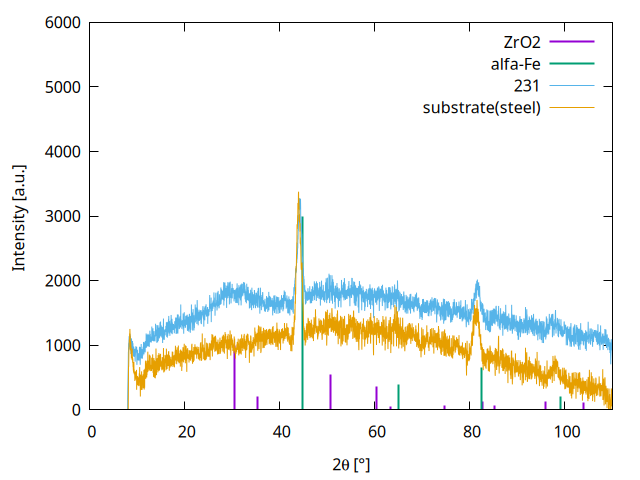
\includegraphics[width=\picwidth]{Pics/xrd.png}
	\caption{XRD spectra of steel substrate (yellow; below), \gls{zro} (blue; above), $\alpha$-Fe (green; wide; idealized) and cubic-\gls{zro} (purple; narrow; idealized)\cite{gkatz1971xray} }%\td{(text in fig too small, use an offset, looks very amorphous to me)} }
	\label{fig:xrd}
	% 207_6113_10x2F_v18T40_T500v2
\end{figure}

\Gls{xrd} was used in order to confirm that the produced layer is indeed \gls{zro}. 
Figure~\ref{fig:xrd} shows diffractograms of the substrate (steel) and 
the substrate with ten layers of double concentrated solution (\gls{emma} experiment number 6113, see Appendix~\ref{sec:app-emma}).
In addition, two idealized diffractograms from the Crystallography Open Database of cubic \gls{zro} (COD ID 1521753\cite{gkatz1971xray}) and of $\alpha$-Fe (COD ID 1100108) are depicted.
%
The four largest peaks of the cubic \gls{zro} reference diffractogram at $2\theta=$ \ang{30}, \ang{51}, \ang{60}, \ang{35} (highest to lowest intensity) can also be observed in the experimental diffractogram. %. clearly stand out against the noise from the experimental diffractogram.
They confirm that the coated material is indeed \gls{zro}.
Raman spectra are needed to further clarify the phase, 
since cubic and tetragonal phases are difficult to distinguish from \gls{xrd} alone\cite{Purohit2006Combustion}.

%%%%%%%%%%%%%%%%%%%%%%%%%%%%%%%%%%%%%%%%%%%%%%%%%%%%%%%%%%%
%%%%%%%%%%%%%%%%%%%%%%%%%%%%%%%%%%%%%%%%%%%%%%%%%%%%%%%%%%%
\subsection{Spectrometry of \ch{ZrO2} Layers}
%\todo{of what?}
\begin{figure}[htb]
    \centering
    \begin{subfigure}{.49\textwidth}
        \centering
        \includegraphics[width=.99\textwidth]{Pics/ir-gt.png}
		\caption{}%Transmission of \gls{zro} on glass} 
		\label{fig:ir-gt}
    \end{subfigure}
    \begin{subfigure}{.49\textwidth}
        \centering
        \includegraphics[width=.99\textwidth]{Pics/ir-gr.png}
		\caption{}%Reflection of \gls{zro} on glass} 
		\label{fig:ir-gr}
    \end{subfigure}
	\label{fig:ir}
	\caption{UV/Vis/NIR spectra of different \gls{zro} layer counts on glass 
	(a)~transmission at \SI{0}{\degree} and (b)~reflection at \SI{45}{\degree} 
	} 
%	"138_g_00L_R.dpt"  w l t "0"  , \
%	"118_g_03L_R.dpt"  w l t "3"  , \
%	"114_g_05L_R.dpt"  w l t "5"  , \
%	"130_g_10L_R2.dpt" w l t "10" , \
%	"136_g_11L_R.dpt"  w l t "11"
%	Reflection vs Reflectance and Transmission vs Transmittance
\end{figure}

In figure~\ref{fig:ir-gt} \gls{uv}/\gls{vis}/\gls{nir} transmittance spectra of \gls{zro} layers on glass slides can be seen. 
Each sample had different numbers of coated layers. 
The incident angle was \ang{0} for each sample.
%differnt numbers of layers of \gls{zro} on a glass slide with 0 degree incident angle. 
The more layers, the more of the light is absorbed (at 600-\nm{1100}) by the \gls{zro} layers. 
%The trend is not monotonic due to inhomogenities in the sample???b
The thicker the layer is, the more wavy the graph, which can be attributed to interference\cite{Dumin1967}.
This trend can also be observed in figure~\ref{fig:ir-gr}.
The weak interference patterns at low wavelengths indicate that the thickness of the film is in the order of magnitude of the wavelengths\cite{delimafilho2017film} -- agreeing with \gls{sem} measurements. 
%
Figure~\ref{fig:ir-gr} shows reflectance spectra of \gls{uv}/\gls{vis}/\gls{nir} at an incident angle of \ang{45}. 
%The shift of the wavy part of the spectra (comparing reflectance with transmittance) can be explained by the longer path of light through the \gls{zro} layer because of the incident angle. 
Thicker layers reflect more light between approximately \nm{800} and \nm{1000}. 
Again, this effect is most likely not observed across the whole spectrum because of interferences. 
%It is interesting to note the shoulder at around \nm{850} present in every spectrum.


%%%%%%%%%%%%%%%%%%%%%%%%%%%%%%%%%%%%%%%%%%%%%%%%%%%%%%%%%%%
%%%%%%%%%%%%%%%%%%%%%%%%%%%%%%%%%%%%%%%%%%%%%%%%%%%%%%%%%%%
\subsection{Current Voltage Curves of \ch{ZrO2} Layers} 
%\todo{of what?}
\begin{figure}
    \centering
	%
    \begin{subfigure}{.32\textwidth}
        \includegraphics[width=.99\textwidth]{Pics/iv/log-154-good-3x4F.png}
		\caption{}%log good 3x4F} 
		\label{fig:iv-log-good}
    \end{subfigure}
    \begin{subfigure}{.32\textwidth}
        \includegraphics[width=.99\textwidth]{Pics/iv/log-146-okay-10x1F.png}
		\caption{}%log okay 10x1F} 
		\label{fig:iv-log-okay}
    \end{subfigure}
    \begin{subfigure}{.32\textwidth}
        \includegraphics[width=.99\textwidth]{Pics/iv/log-156-bad-3x3F.png}
		\caption{}%log bad 3x3F} 
		\label{fig:iv-log-bad}
    \end{subfigure}
	%
    \begin{subfigure}{.32\textwidth}
        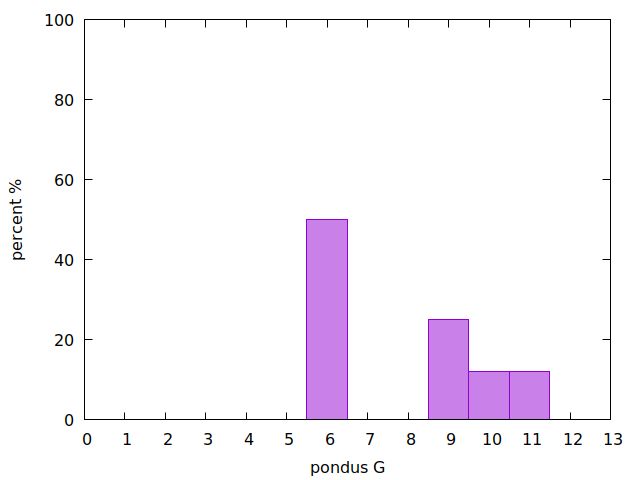
\includegraphics[width=\textwidth]{Pics/iv/stat-154-okay-3x4F.png}
		\caption{}%stat good 3x4F} 
		\label{fig:iv-stat-good}
    \end{subfigure}
    \begin{subfigure}{.32\textwidth}
        \includegraphics[width=\textwidth]{Pics/iv/stat-146-good-10x1F.png}
		\caption{}%stat okay 10x1F} 
		\label{fig:iv-stat-okay}
    \end{subfigure}
    \begin{subfigure}{.32\textwidth}
        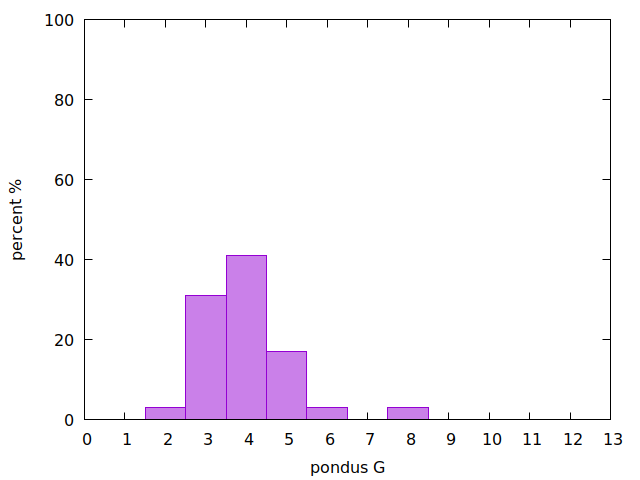
\includegraphics[width=\textwidth]{Pics/iv/stat-156-bad-3x3F.png}
		\caption{}%stat bad 3x3F} 
		\label{fig:iv-stat-bad}
    \end{subfigure}
	%
    \begin{subfigure}{.32\textwidth}
        \includegraphics[width=\textwidth]{Pics/iv/146-nocurrent.png}
		\caption{}%no current} 
		\label{fig:iv-nocurrent}
    \end{subfigure}
    \begin{subfigure}{.32\textwidth}
        \includegraphics[width=\textwidth]{Pics/iv/146-diodic.png}
		\caption{}%diodic} 
		\label{fig:iv-diodic}
    \end{subfigure}
    \begin{subfigure}{.32\textwidth}
        \includegraphics[width=\textwidth]{Pics/iv/146-ohmic.png}
		\caption{}%ohmic} 
		\label{fig:iv-ohmic}
    \end{subfigure}
	%
%    \caption{\td{maybe remove 146 and make 154 good AND set yrange [E-1:E-14] and show phd threshold}} \label{fig:iv}
	\caption{
		Current-voltage curves and the distribution of gradients for three representative samples: insulating well (a),(d),(g), moderately (b),(e),(h), poorly (c),(f),(i); 
		(a)-(c) I-V curves with log transformed current; 
		(d)-(f) frequency histograms of the conductance with pin hole threshold marked as vertical line; 
		(g)-(i) individual I-V measurements
	}
    \label{fig:iv}
\end{figure}

%Figures~\ref{fig:iv-log-good} and~\ref{fig:iv-stat-good} are measurements from a good sample. 
%Figure~\ref{fig:iv-log-good} shows \gls{iv} curves in logarithmic scale of an insulating sample. 
Figure~\ref{fig:iv-log-good} shows \gls{iv} curves of an insulating sample, where the abscissa shows the voltage in Volt and the ordinate shows the current in Ampere. 
Each line represents a I-V measurement at a distinct aluminium contact applied by sputtering through a mask (see figure~\ref{fig:micro}).
All of the curves show a max voltage of under \num{e-6} \SI{}{\volt} 
and around a fifth exhibit hardly any current, which is ideal (see figure~\ref{fig:iv-stat-good}).
A single example for a very low conductance measurement in non-logarithmic scale can be seen in figure~\ref{fig:iv-nocurrent}.
The conductance (i.e. the gradient at V=0) was calculated (see section~\ref{sec:eval}) for each measurement.
Figure~\ref{fig:iv-stat-good} shows the distribution of gradients $g$ for the same sample as depicted in \ref{fig:iv-log-good}.
%
Figures~\ref{fig:iv-log-okay} and~\ref{fig:iv-stat-okay} show measurements of a moderately insulating sample. 
Most of the \gls{iv} curves have a maximum voltage of under \num{e-6}\SI{}{\volt}, 
but there are some pinholes with conductance above the threshold of \num{e-5}\SI{}{\volt}. %\num{e-6} V. 
%
In figures~\ref{fig:iv-log-good} and~\ref{fig:iv-log-okay} the minimum of some curves 
is not at \SI{0}{\volt}, which means that the function does not cross the origin in non-logarithmic representation. 
%
This deviation (see figure~\ref{fig:iv-diodic}) looks similar to the deviation due to the photo-currents\cite{perez2018solar} because of its non-zero current at $V=0$.
%, but was not investigated further. 
Though, the explanation by photo-current is compelling, it does most likely not apply because of \gls{zro}'s band gap of \ev{5}\cite{sinhamahapatra2016oxygen}.
A better explanation would be the tunneling effect, whose \gls{iv} curves look very similar\cite{feenstra1994scanning,datta1997current}.
%\td{show some non log \gls{iv} curves and discuss form, some look like tunneling\cite{feenstra1994scanning,datta1997current}.}
%
Finally, figures~\ref{fig:iv-log-bad} and~\ref{fig:iv-stat-bad} show a sample 
where all measurements exhibit relatively high voltages and high calculated conductances. 
This indicates a overall bad condition of the \gls{zro} layer for insulating. 
Figure~\ref{fig:iv-ohmic} shows a \gls{iv} curve which can be approximated by Ohm's law. 
%

%%%%%%%%%%%%%%%%%%%%%%%%%%%%%%%%%%%%%%%%%%%%%%%%%%%%%%%%%%%
%%%%%%%%%%%%%%%%%%%%%%%%%%%%%%%%%%%%%%%%%%%%%%%%%%%%%%%%%%%
\subsection{Pre-optimization of Coating Procedure}
%\todo{of what?}
Before the optimization with the \gls{emma} algorithm, 
the boundaries of the input variables were explored. 
Especially, the \gls{db} velocity $v_{C}$ (i.e. the velocity with which the blade moves and spreads the solution over the sample)
was varied and examined during pre-optimization. 
The slower the \gls{db} velocity, the more uniformly the solution evaporated. 
If the $v_{C}$ was too slow (less than \mmps{1}), no \gls{zro} layer was formed. 
The reason could be that the force exerted by the blade on the liquid is not strong enough to overcome the combination of gravity and the surface tension of the alkoxide solution.
This means that behind the blade a meniscus would pull the liquid without leaving behind any solution for the gelling process. 
Additionally, the coating temperature affects the evaporation process together with the \gls{db} velocity $v_{C}$. 

%\td{Assumption: Ideally solution evaporate shortly after DB but not before}
%due to the boiling point of \gls{buoh} at 117 C\cite{ncbi1butanol} the room temperature to 80 C were used as temperature during \gls{db}.
%- p76, 146 (10x1F) good, 154 (3x4F) okay, 156 (3x3F) bad visualization

%%%%%%%%%%%%%%%%%%%%%%%%%%%%%%%%%%%%%%%%%%%%%%%%%%%%%%%%%%%
%%%%%%%%%%%%%%%%%%%%%%%%%%%%%%%%%%%%%%%%%%%%%%%%%%%%%%%%%%%
%\subsection{SEM}

%The \gls{sem} pictures were not easy to take since 
%it has been tried to create an insulator 
%and the quality of the picture relies on the conductance of the material's surface. 
%This means that the better the quality of the resulting layer the more tedious it was to take a decent SEM image. 

%
%5F ca 100min
%4F ca 140min
%3F ca 420min (7h)
%extra AcOH stabilzed but needed so much that dilution too large...
%\td{IPO influence on "stability" p74: 600ul IPO makes clear, 4000 ul BuOH not clear with 
%same base solution (1ml of 4F), added extra 400ul to BuOH sol and after 5min clear. 
%of 1:5 is unacceptable Dilution }
%- 21.8 (1F) from 15.02. 13:30 bis 
%26.3 (1ml iPO to ca2ml of 5f) from 16.02. 16:30 bis 18.02.++
%18.02 4F in 80min milky
%      2F in ca 24h (stabilization AcOH)
%
%acceptable layer was produced by buthanolic solution, but very unstable (short lived) how long? p41 
%\Gls{ipo} solution allowed to even reuse high concentrated solution, which would otherwise become cloudy under 60 minutes. 
%Multiple question still need to be answered: 
%What causes the cloudiness (as stability increased through sealing probably \ch{H2O} from the air or \ch{O2}) and what's the mechanism? 
%How does \gls{ipo} increase the stability? 
%Does it do so because it "fits" better with the solvent. 
%As the original solvent was 2-methoxy-ethonanol instead of \ch{buoh}. 
%It was even observed that the addition of \td{some drops of} \gls{ipo} to an acetic solution can clear the solution.
%5F acetic solution milky over night 5:1 dilution with \gls{ipo} and clear after one minute of stirring and stayed clear over 5 nights.
% more details on pages 68ff
%No effect on the solution or the resulting layer was noticed \td{from the initial stirring}
%\todo{Following stirring times (in minutes) were tested and didn't have an influence on stability of the solution: 10-10-20, 10-10-45, 30-30-180.}
%The stirring time was untersucht, but not much difference so shortest was used because 
%short time can produces faster and the resulting solution is longer stable 
%(after finishing mixing)

%\td{instead of changing the stabilization agent before optimization, could change after pso, was vor und nachteile?}
%after realizing the improved effectiveness of \gls{ipo} for experimentation, 
%it was decided that EMMA will be executed with \gls{ipo} solution.


%- first recipe tried to improve to achieve more resisting layer. 
%by pH value, surface tension and solution ratios 
%(only 10\% change because it was assumed, that the recipe is good and should be improved, 
%but the recipe should be altered thoroughly. 
%two layers were also tried but didn't even pass the visual examination/test/inspection. 
%A curst was produced. 
%It is assumed 

%\iffalse
%\begin{figure}
%    \centering
%    \begin{subfigure}{.45\textwidth}
%        \centering
%        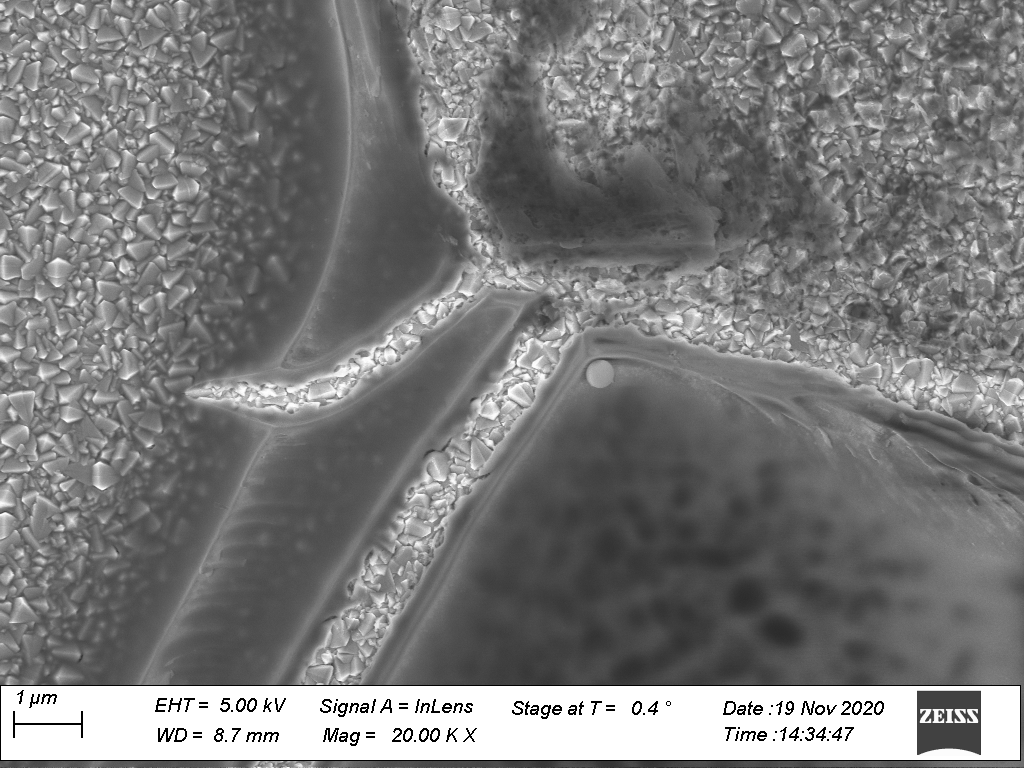
\includegraphics[width=.8\textwidth]{Pics/sem/071_fto_old_1x.png}
%        \caption{71 fto old 1x} \label{fig:sem-old1}
%    \end{subfigure}
%    \begin{subfigure}{.45\textwidth}
%        \centering
%        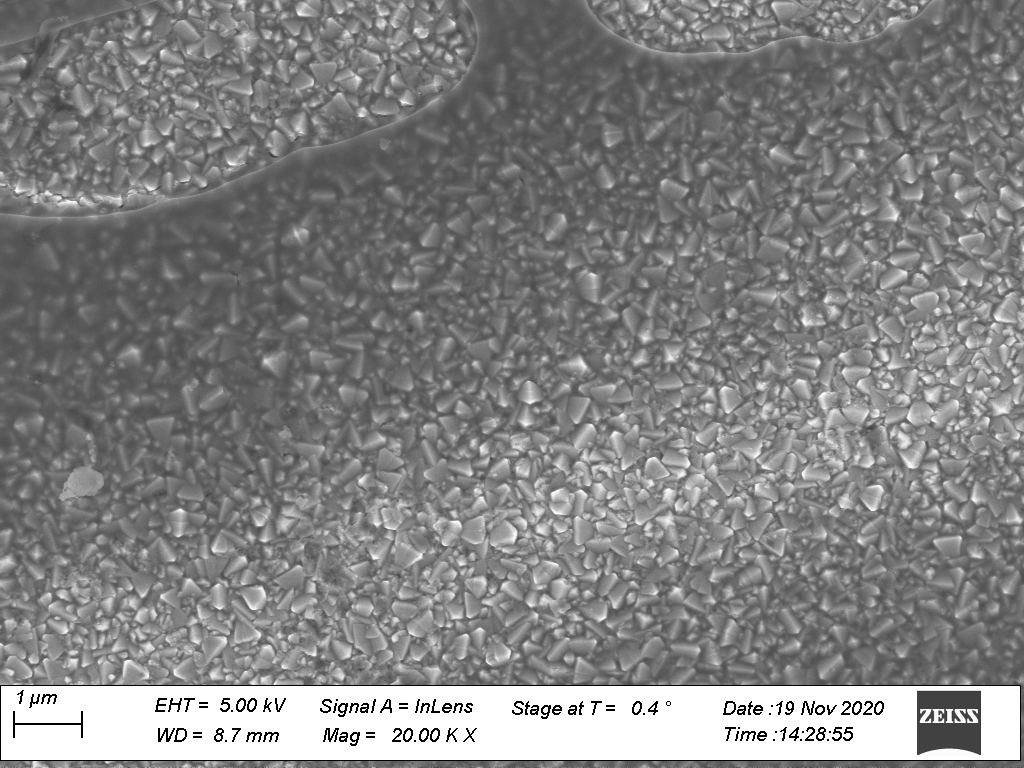
\includegraphics[width=.8\textwidth]{Pics/sem/071_fto_old_2x.png}
%        \caption{71 fto old 2x} \label{fig:sem-old2}
%    \end{subfigure}
%    \begin{subfigure}{.45\textwidth}
%        \centering
%        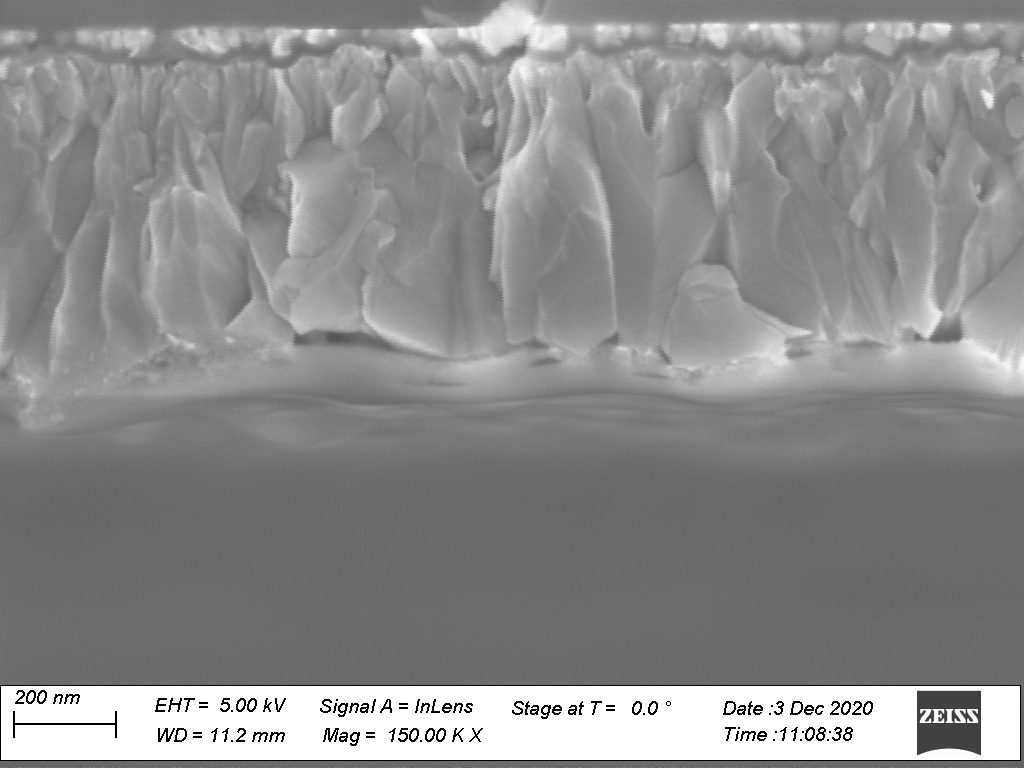
\includegraphics[width=.8\textwidth]{Pics/sem/115_fto_cs_1x.png}
%        \caption{115 fto cs 1x} \label{fig:sem-cs1}
%    \end{subfigure}
%    \begin{subfigure}{.45\textwidth}
%        \centering
%        %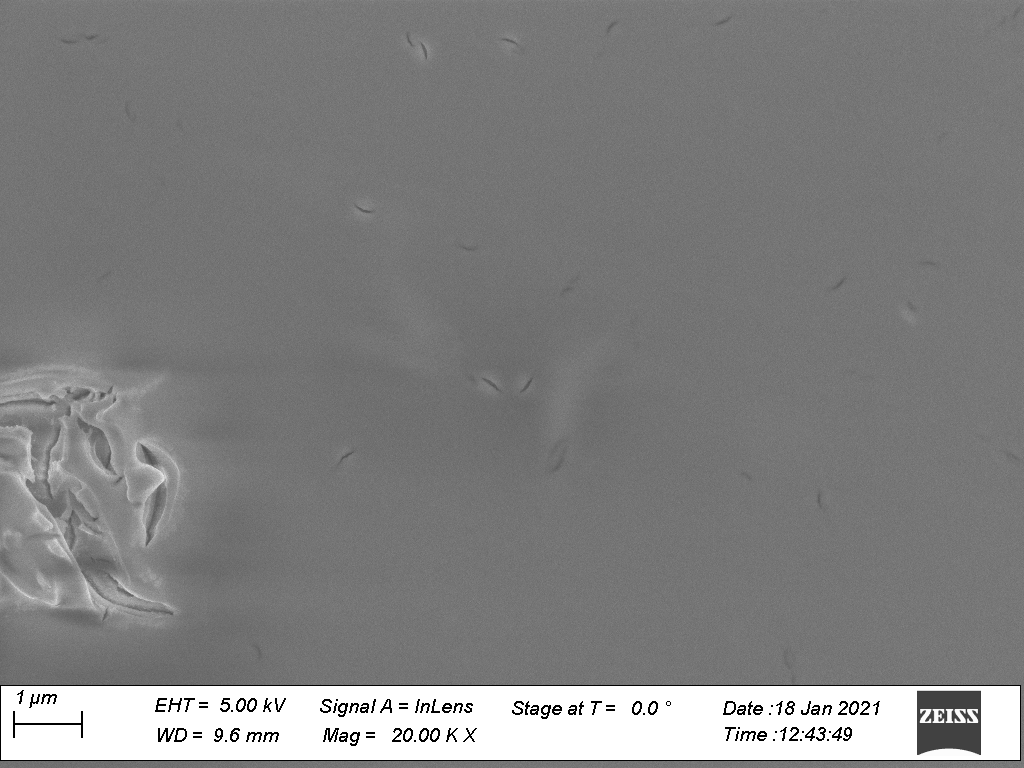
\includegraphics[width=.8\textwidth]{Pics/sem/147_steel_ph_10x.png}
%        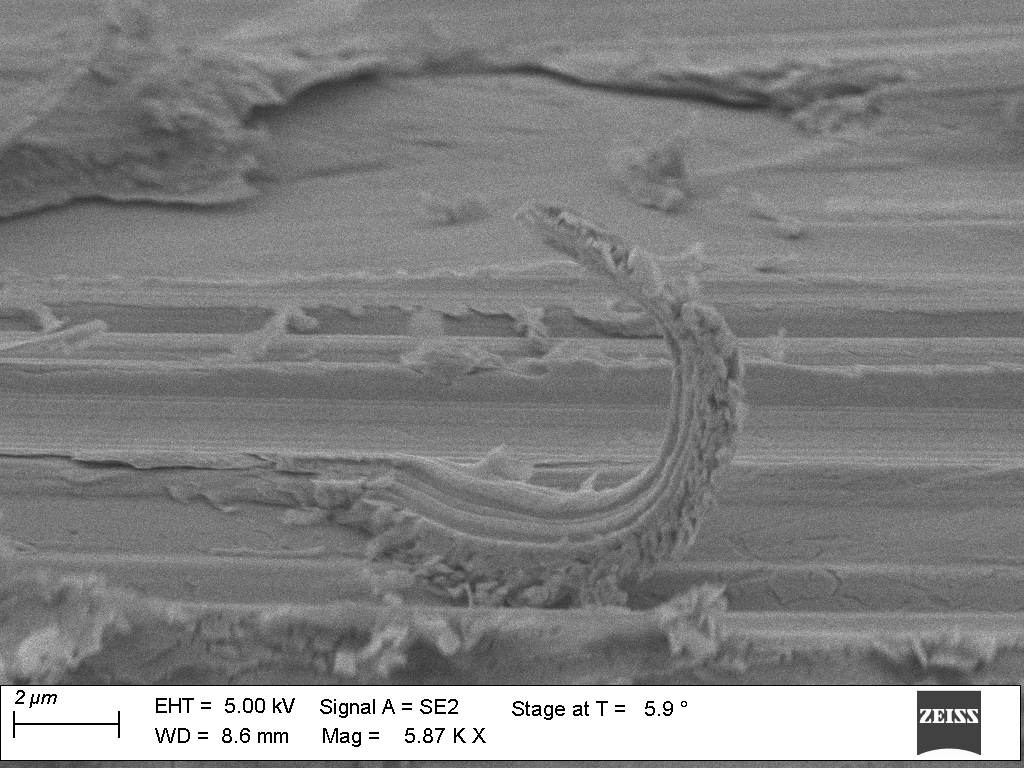
\includegraphics[width=.8\textwidth]{Pics/sem/150_steel_cs_2Fx5.png}
%        \caption{150 steel 2Fx5} \label{fig:sem-cs2}
%    \end{subfigure}
%    \caption{cross section}
%    \label{fig:sem}
%\end{figure}
%\fi


%\iffalse
